% Activate the following line by filling in the right side. If for example the name of the root file is Main.tex, write
% "...root = Main.tex" if the chapter file is in the same directory, and "...root = ../Main.tex" if the chapter is in a subdirectory.

\chapter{Introduction}

Many undergraduate Mathematics programs require students to take 
a proof-writing course, as proofs insert formal rigor into the 
study of Mathematics. Still, there’s some degree of uncertainty, 
since human error is involved in evaluating the proofs and 
determining their consistency. For 
simpler proofs, the risk of human error is a lesser problem, 
since a discerning eye can quickly catch holes in a faulty proof. 
Nonetheless, grading the quality of a slew of proofs is 
time-consuming, especially when factoring in the time a grader 
might take to provide feedback for the specific errors in a 
poorly-written proof. Students may also have difficulty
determining how much detail is sufficient for the proofs they
write, if they even notice the holes in their proofs. For 
both instructors and students, the ambiguity in what constitutes
a ``formal proof'' adds work outside of the mathematical and 
logical focus of the course.

Theorem provers and proof assistants can help resolve this ambiguity,
using the determinism of computing. Theorem provers verify that
the proofs encoded in the prover are sound, namely that they follow
from the axioms and rules of inference. The rigorous framework
of formal mathematics is thus supported by automation which can, 
for students, provide immediate feedback, 
and for instructors, grade instantly and without bias.

One such theorem prover, Lean,
uses dependent type theory and the Curry-Howard isomorphism 
to build a programming language capable of defining and proving 
theorems in Mathematics \cite{TPiL}. Lean stands out when compared to other
theorem provers like Coq and Isabelle due to Lean's
extensive math library, Mathlib, and its large active community 
of users. Lean also has a “tactic mode,” wherein all of the 
premises and goals of a proof are displayed 
as they develop throughout the proof, and functions called 
“tactics” can be used to advance through the proofs using 
automation and type inference. Lean’s large user base and 
committed development team have also created a variety of 
supplemental resources for new users to learn Lean and for 
experienced users to reference, most notable of which is 
\textit{Mathematics In Lean} \cite{MIL}.

\textit{Mathematics In Lean} (MIL) was the primary resource I used 
to learn Lean, and I found the textbook to be a smooth
onramp for a student like myself with a few years of undergraduate
math and computer science education. However, I found the textbook
significantly harder to use once the mathematics being introduced 
expanded beyond what I had already studied. For an audience without
much (or any) proof-based mathematics experience, MIL would be 
far too challenging for a first introduction to formal proof.
As an alternative resource, I have developed a throroughly-commented
interactive code library designed to teach undergraduate Mathematics
students the basics of formal proof-writing, set theory, and topology 
with the assistance of Lean \cite{GrenierLIT}. The code library covers first-order logic,
introductory set theory, order and equivalence relations, induction, and
some point-set topology. 

\begin{wrapfigure}{r}{0.5\textwidth}
    \caption{My GitHub Library}
    \centering
    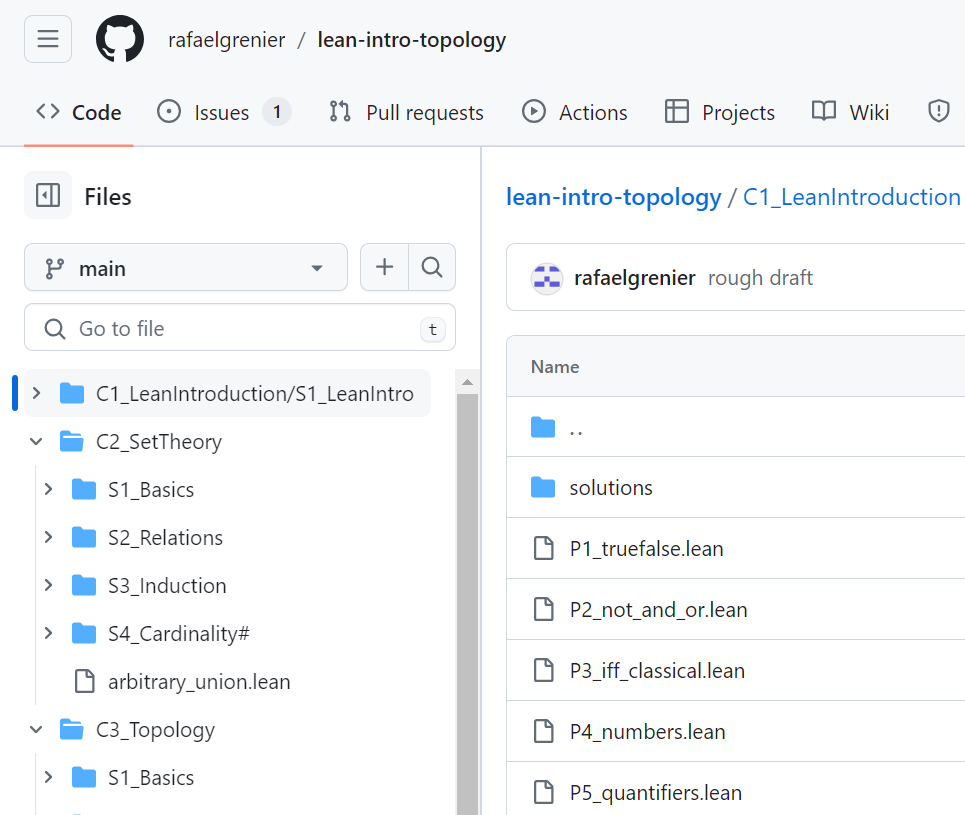
\includegraphics[width=0.5\textwidth]{Chapter1/repo.png}
\end{wrapfigure}

The section \lean{S1\_LeanIntro} of the first chapter \lean{C1\_LeanIntroduction} introduces propositions, 
logical connectives, predicates, quantifiers, and just enough
type theory to begin working with Lean. 

The second chapter \lean{C2\_SetTheory} starts with the section
\lean{S1\_Basics} which introduces sets, set operations like union and intersection,
functions, and cartesian products.
The section \lean{S2\_Relations} considers two kinds of relations:
order relations and equivalence relations. The order relations
discussed are preorder, partial order, lexicographic order, and 
strict order. The introduction to equivalence relations transitions 
to equivalence classes, set/type partitions, and quotients. 
The section \lean{S3\_Induction}
brings in weak and strong induction, as well as inductive
types and recursive definitions.

The third chapter \lean{C3\_Topology} has the final section \lean{S1\_Basics}
on point-set topology which introduces the definition of a 
topology, a topological basis, and open/closed sets. Then the section
pivots to the order, subspace, and product topologies.

This code library was my honors thesis project, and this paper
will explain the structure of the code library, the process of
developing it, and the conclusions I came to as a result.
